% Miktex Beamer template
% Author: Carl Schneider
% University TUDelft
% www.dutiosc.twi.tudelft.nl/~carl/
% or: http://www.ewi.tudelft.nl/live/pagina.jsp?id=3b29bfdd-1cb1-4e15-b03c-a5dab56837e2&
% April 2010

\documentclass{beamer}

% Necessary definitions:
\setbeamersize{sidebar width left=0.5cm}
%\usepackage[english]{babel}
\usepackage{tikz}
\usepackage[utf8]{inputenc}
\newcommand{\field}[1]{\mathbb{#1}}
\newcommand{\Zset}{\field{Z}}
\mode<presentation>
{\usetheme{Boadilla} % This theme will be adjusted into the TUDelft lay-out
 \setbeamercovered{transparent}}
\definecolor{tudblue}{rgb}{.004,.50,.78} % definition TUDelft blue color
\setbeamercolor{structure}{fg=tudblue}
\setbeamercolor{palette primary}{fg=white,bg=tudblue!85}       % Right field
\setbeamercolor{palette secondary}{fg=white,bg=tudblue!85}     % Middle field
\setbeamercolor{palette tertiary}{fg=tudblue!85,bg=tudblue!85} % Left field
\setbeamersize{text margin left=1cm}
\setbeamersize{text margin right=1cm}

%---------------------------------------------------------------------------------
%  Take attention for the parts you may change. See the comment lines with: %>>>
%---------------------------------------------------------------------------------

%>>> You may change the text in this part {Between brackets}:
%>>> This is for the Title page:
\newcommand*\titel{The Open Society}
\newcommand*\subkop{A Concise Synopsis}
\newcommand*\naam{Martin Jorn Rogalla}
\newcommand*\afdeling{EEMCS}
%>>> This is for the frame-title on the "Table of Contents" page:
\newcommand*\titelTOC{Outline}
%>>> This is for the frame-title on the "Table of Contents" page when the next subsection will start:
\newcommand*\subsectie{Next Subsection}


%%% Not change this part below %%%
%%% Title Page (belongs to the theme)%%%
% Necessary part for the theme:
\title{\titel} % This title also appears in the TUDelft bar on the next pages
\author[]{\naam}
\institute[]{\subkop \\ TU Delft}
\date[]{\today}
\AtBeginSubsection[]
{\begin{frame}<beamer>\frametitle{\textbf{\LARGE{\textrm{\subsectie}}}}
    \tableofcontents[currentsection,currentsubsection]  % Generation of the Table of Contents
\end{frame}}
\tikzset{textlabel/.style={color=white}}
\beamertemplatetransparentcovereddynamicmedium

%==============================================================
%%% Not change this part below, except maybe the folder where you placed the "TUDelft bies"
\begin{document}
% Adjusting boadilla theme lay-out to TUDelft lay-out:
\setbeamertemplate{sidebar left}  % blue square left above
{\vfill
\rlap{%\hskip0.1cm

\includegraphics[scale=0.33]{TUDelft/beamer-tudelft-bies.jpg} }
\vskip-5pt}

%--------------------------------------------------------------

% Section 0
% Subsection 0
% Page 1
% Title page
%%% This is the first frame of the presentation.
%%% Please do not change it except maybe the comment signs in case of a background photo
%%% and the place and name of the photo (
\begin{frame}
    \begin{tikzpicture} [remember picture, overlay]
        \node [shift={(0.5 cm,-5.35cm)}]  at (current page.north west)
        {
        \begin{tikzpicture}[remember picture, overlay]
            %%% These 2 coming lines you may uncomment if you want to have a photo on the background(2198x1480pixels) of the title page
            \node [shift={(-0.14cm,5.56cm)},right] at (current page.south west) % background photo
            {
\includegraphics[height=8.65cm]{TUDelft/background-titlepage.jpg}};            % background photo
            \fill [cyan!95!black!70!blue] (0,2.9) -- (0,5.35) -- (-.5,5.35) -- (-.5,2.9) -- cycle ;%squareNorthWest
            \draw [fill=black] (0,0) -- (11,0) -- (11,2.9) -- (0,2.9) -- cycle ;
            \fill [fill=cyan!65!blue!80] (7,-3.9) -- (12.4,-3.9) -- (12.4,-3.65) -- (7,-3.65) -- cycle;
            \node [shift={(0.8cm,-2.9cm)},textlabel,right]  at (current page.north west) {\textbf{\LARGE{\textrm{\titel}}}};
            \node [shift={(0.8cm,-3.5cm)},textlabel,cyan!95!black!70!blue,right]  at (current page.north west)
            {\textbf{\large{\textrm{\subkop}}}};
            \node [shift={(0.8cm,-4.6cm)},textlabel,right]  at (current page.north west)
            {\normalsize{\naam, \afdeling}};
            \node [shift={(0.8cm,-5cm)},textlabel,right]  at (current page.north west)
            {\normalsize{\today}};
        \end{tikzpicture}};
    \end{tikzpicture}
\end{frame}

%--------------------------------------------
%%% Table of contents (TOC)
% The TOC will generated after building your section(s) and subsections
\begin{frame}<beamer>\frametitle{\textbf{\LARGE{\textrm{\titelTOC}}}}
    \begin{tikzpicture}[remember picture, overlay]
        \node [shift={(0.5 cm,-5.35cm)}]  at (current page.north west)
        {
        \begin{tikzpicture}[remember picture, overlay]
            \fill [fill=cyan!65!blue!80] (7,-3.9) -- (12.4,-3.9) -- (12.4,-3.65) -- (7,-3.65) -- cycle;
        \end{tikzpicture}};
    \end{tikzpicture}
    \tableofcontents
\end{frame}
%--------------------------------------------

\section{Fallibilism}

\begin{frame}\frametitle{\textbf{\LARGE{\textrm{Fallibilism - Karl Popper}}}}
  \begin{figure}
    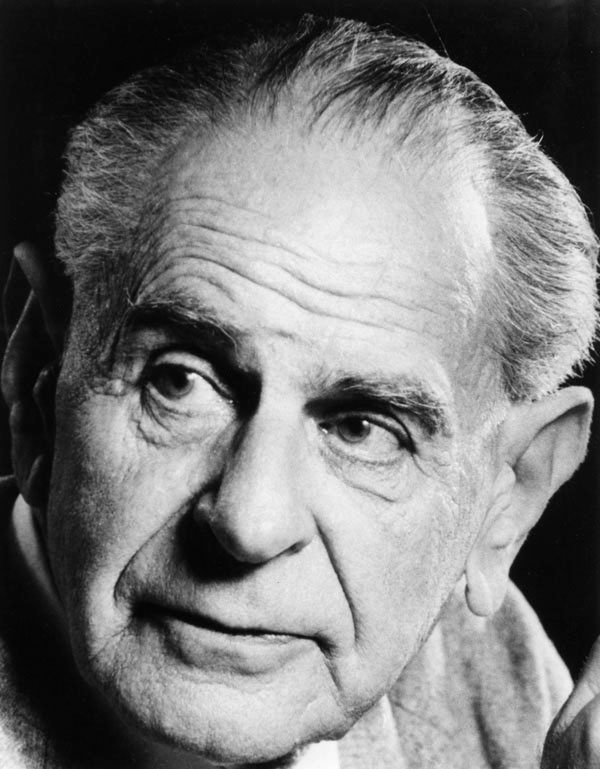
\includegraphics[height=3cm]{images/Karl_Popper.jpg}
  \end{figure}
  \begin{itemize}
    \item Seen as one of the founders of the Open Society.
    \item Emphasized the importance of formulating uncertainty in scientific theories(Fallisism).
    \item Wrote the book "The Open Society and its Enemies"
  \end{itemize}
\end{frame}

\begin{frame}\frametitle{\textbf{\LARGE{\textrm{Fallibilism - Definition}}}}
The philosophical principle that human beings could be wrong about their beliefs, expectations, or their understanding of the world. 
\end{frame}

\begin{frame}\frametitle{\textbf{\LARGE{\textrm{Fallibilism - Concrete Sense}}}}
In the most commonly used sense of the term, this consists in being open to new evidence that would 
disprove some previously held position or belief, and in the recognition that ``\emph{any claim justfied today 
may need to be revised or withdrawn in light of new evidence, new arguments, and new experiences.}''\cite{kompridis2006critique}
\end{frame}

\begin{frame}\frametitle{\textbf{\LARGE{\textrm{Fallibilism vs. Skepticism}}}}
Fallibilism is the \emph{epistemological} stance that what we think of as knowledge is subject to refutation. 
Skepticism is the position that attaining knowledge is not possible.
\end{frame}

\section{Open Society}
\begin{frame}\frametitle{\textbf{\LARGE{\textrm{Open Society - Definition}}}}
Popper defined the open society as one ``in which individuals are confronted with personal decisions'' as opposed to a ``magical or tribal or collectivist society.''\cite{popper2011open}
\end{frame}
\begin{frame}\frametitle{\textbf{\LARGE{\textrm{Open Society - Definition Extended}}}}
A society characterized by a flexible structure, freedom of belief, and wide dissemination of information.
\end{frame}

\section{Open-Source Governance}
\begin{frame}\frametitle{\textbf{\LARGE{\textrm{Open-Source Governance - Definition}}}}
 A political philosophy which advocates the application of the philosophies of the open source and open content movements to democratic principles in order to enable any interested citizen to add to the creation of policy, as with a wiki document.
\end{frame}

\begin{frame}\frametitle{\textbf{\LARGE{\textrm{Open-Source Governance - Results}}}}
Legislation is democratically opened to the general citizenry, employing their collective wisdom to benefit the decision-making process and improve democracy.
\end{frame}

\section{Finalization}
\begin{frame}\frametitle{\textbf{\LARGE{\textrm{Discussion}}}}
\begin{enumerate}
  \item Direct democracy is the best solution to governing our society.
  \item For the sake of National Security, legislation on the capabilities of the National Security Agency is not be made public.
  \item Voting should be made compulsory.
  \item Prisoners should not be allowed to vote.
  \item If I disagree with the way the voting system is set, I should not vote to show my discontent.
\end{enumerate}
\end{frame}

\begin{frame}[allowframebreaks]
  \frametitle<presentation>{Bibliography}    
  \begin{thebibliography}{10}    
  \beamertemplatebookbibitems
  \bibitem{kompridis2006critique}
    Kompridis,~Nikolas
    \newblock {\em Critique and disclosure: Critical theory between past and future}.
    \newblock MIT Press Cambridge, 2006.
  \beamertemplatebookbibitems
  \bibitem{popper2011open}
    K.~Popper.
    \newblock {\em The open society and its enemies}.
    \newblock Routledge
  \end{thebibliography}
\end{frame}

\end{document} 
